\section{Materiales y métodos}
\subsection{Single View Metrology in the Wild}
\begin{frame}
    \frametitle{Single View Metrology in the Wild}
    \begin{figure}[!ht]
      \center
      \includegraphics[width=.65\textwidth]{imagenes/chapter2/scene_model.pdf}
      \caption{Modelo de escena de Rui Zhu \emph{et al}\footnotemark}
    \end{figure}
    \footcitetext{SVMIW}
\end{frame}

\note{
No obstante, nuestro enfoque será en el que más encaja con nuestro título
``Single View Metrology in the Wild'' de Zhu et al.
En él, argumentan poder estimar la escala absoluta de la imagen entrenando
en datos no supervisado que nos permita modelar ciertas variables del modelo de escena que se
dibuja en pantalla. Es el modelo típico proyectivo de una cámara estenopeica.
La idea es simple en teoría, si logramos estimar ciertos parámetros sencillos de la escena,
como el ángulo de rotación de la cámara con respecto al horizonte, así como detectar las personas
y la caja que las encierra, podremos jugar a hacer re-proyecciones entre las escenas
que nos dará la información de la altura de los objetos en escala absoluta.
}

\begin{frame}
    \frametitle{Single View Metrology in the Wild}
    \begin{enumerate}
      \item Utilizando geometría perspectiva obtenemos las siguientes ecuaciones:
    \end{enumerate}
    \vspace{.5cm}
      \begin{equation}
          v_t = \frac{(f\, cos\theta + v_c\, sin\theta)\,h_{obj} + (-f\, sin\theta + v_c\, cos\theta)z - f\,h_{cam}}{h_{obj}tan\theta + z\,cos\theta}
      \end{equation}
      \begin{equation}
        v_b = \frac{-f\,sin\theta z + v_c cos\theta z - f\,h_{cam}}{z\, cos\theta}
      \end{equation}
    \begin{enumerate}
      \item Donde ``$v_t$'' y ``$v_b$'' son la parte superior e inferior de la persona en la imagen.
    \end{enumerate}
    \footcitetext{SVMIW}
\end{frame}

\note{
  -Explicar un poco la ecuación y volver hacia a atrás en la imagen y enseñar "vt" y "vb"
}


\begin{frame}
    \frametitle{Single View Metrology in the Wild}
    \begin{figure}[!ht]
      \center
      \includegraphics[width=1\textwidth]{imagenes/chapter2/pipeline.pdf}
      \caption{Pipeline propuesta por Rui Zhu \emph{et al}\footnotemark}
    \end{figure}
    \footcitetext{SVMIW}
\end{frame}

\note{}

\begin{frame}
    \frametitle{Single View Metrology in the Wild}
    \begin{enumerate}
      \item Las pérdidas adicionales introducidas por el artículo son:
    \end{enumerate}
    \vspace{.3cm}
\begin{equation}
  \mathcal{L}_{vt} ({v_t^i}_{i=1}^N) = \frac{1}{N}\sum_{i=1}^N ||v_{t_{det}}^i - v_t^i||
\end{equation}
\begin{equation}
  \mathcal{L}_{h_{obj}} ({h_{obj}^i}_{i=1}^N) = \frac{1}{N}\sum_{i=1}^N \mathcal{P}(h_{obj}^i;\mu,\sigma)
\end{equation}
        \begin{itemize}
          \item Donde $\mathcal{L}_{v_t}$ es el error de reproyección y $\mathcal{L}_{h_{obj}}$ es el a-priori ($175cm\pm20cm$).
        \end{itemize}
    \footcitetext{SVMIW}
\end{frame}

\subsection{Problemas encontrados}
\begin{frame}
    \frametitle{Problemas encontrados}
    \begin{enumerate}
      \item No está disponible el modelo pre-entrenado por los autores.
      \item No está disponible el código de entrenamiento.
      \item El dataset de calibración de cámara SUN360\footnotemark ya no está disponible públicamente.
    \end{enumerate}
    \footcitetext{SUN360}
\end{frame}

\note{}

\begin{frame}
  \frametitle{Soluciones propuestas}
  \begin{enumerate}
    \item Se ha encontrado un sustituto de SUN360\footcite{SUN360}, PANO360\footcite{SPEC}
      \begin{itemize}
        \item Se obtiene un total de 347.304 imágenes de entrenamiento para estimación de parámetros de cámara.
        \item Para validación se tiene 12.732 imágenes.
      \end{itemize}
    \item Se ha replicado la implementación del artículo utilizando ``detectron2''\footcite{detectron2}.
      \begin{itemize}
        \item Se introduce mejoras de rendimiento y eficiencia a nivel de hardware:
        \item Se simplifica el mantenimiento y extensibilidad del código.
        \item Permite el uso de nuevas arquitecturas y la aplicación de varios avances del campo de visión por computador.
      \end{itemize}
  \end{enumerate}
\end{frame}

\subsection{Datos de entrenamiento}
\begin{frame}
  \frametitle{Datos de entrenamiento: COCO-Scale}
  \begin{itemize}
    \item Subconjunto de imágenes extraídas de COCO~\footcite{COCO}.
    \item 10.547 imágenes de entrenamiento, 2.648 de validación y 584 de test.
    \end{itemize}
\begin{figure}[!ht]
  \begin{center}
    \subfloat{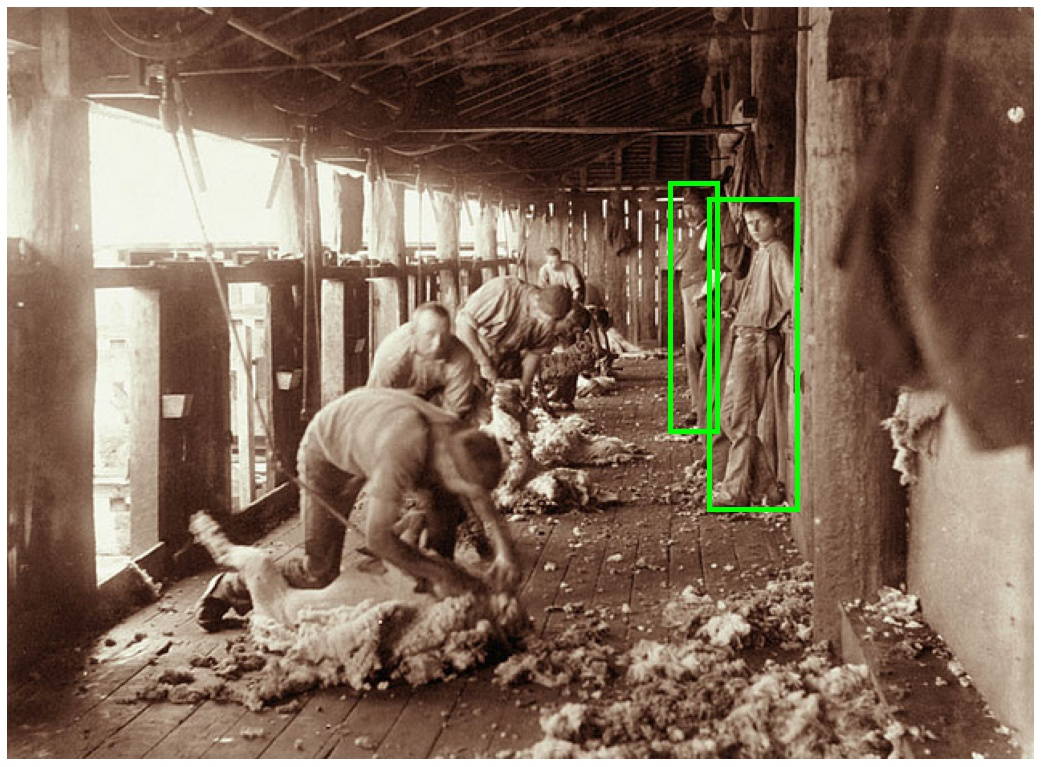
\includegraphics[width=0.25\textwidth]{imagenes/chapter3/COCOScale/sample-000000_reproj.jpg}}
    \subfloat{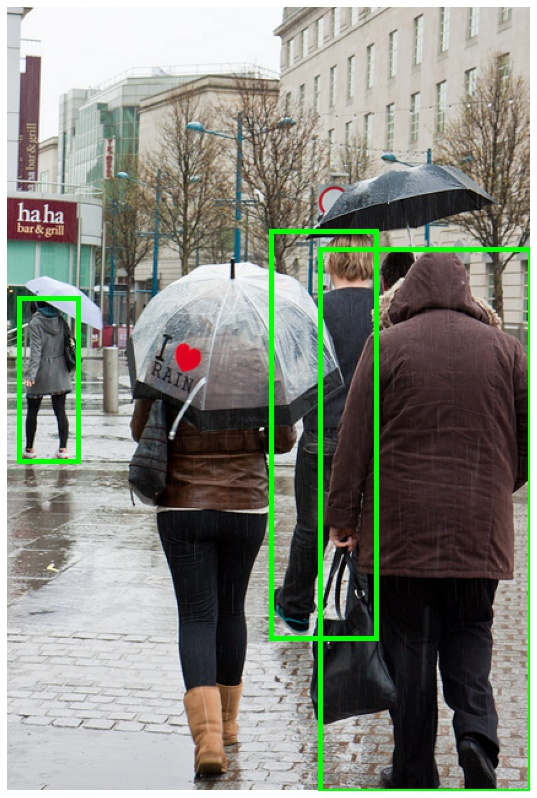
\includegraphics[width=0.12\textwidth]{imagenes/chapter3/COCOScale/sample-000002_reproj.jpg}}
    \subfloat{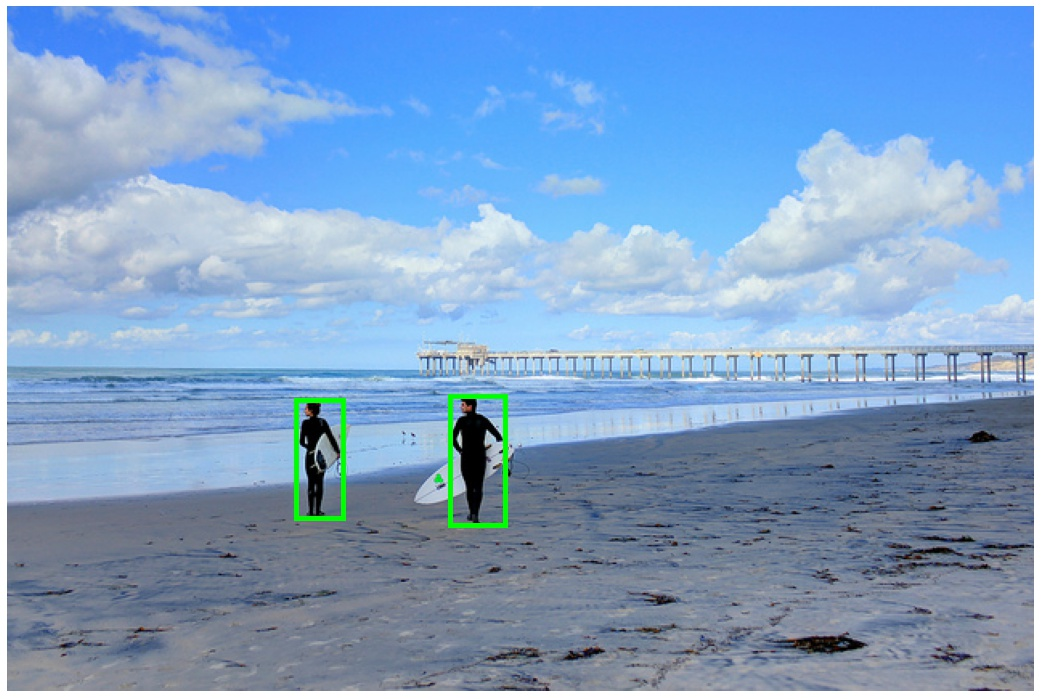
\includegraphics[width=0.25\textwidth ]{imagenes/chapter3/COCOScale/sample-000006_reproj.jpg}}
    \subfloat{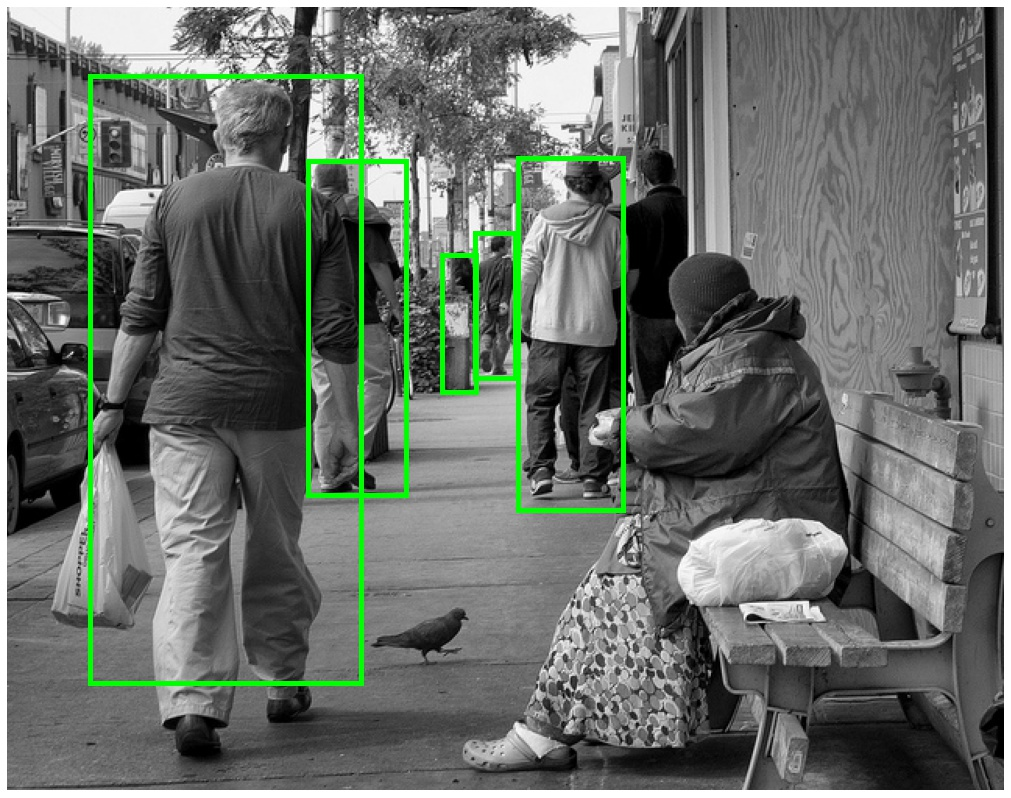
\includegraphics[width=0.25\textwidth]{imagenes/chapter3/COCOScale/sample-000009_reproj.jpg}}
  \end{center}
  \caption[Ejemplos de imágenes extraídas de COCO-Scale~\footcite{SVMIW}.]{
  Ejemplos de imágenes extraídas de COCO-Scale~\footcite{SVMIW}.
  Se observan diferentes tamaños de imagen, rango de colores y las personas detectadas.}
\end{figure}
\end{frame}

\begin{frame}
  \frametitle{Datos de entrenamiento: Pano360}
\begin{figure}[!ht]
  \begin{itemize}
    \item Se obtiene un total de 30033 imágenes de la red social Flickr.
    \item 347.304 imágenes de entrenamiento y 12.732 de validación.
  \end{itemize}
  \begin{center}
    \subfloat{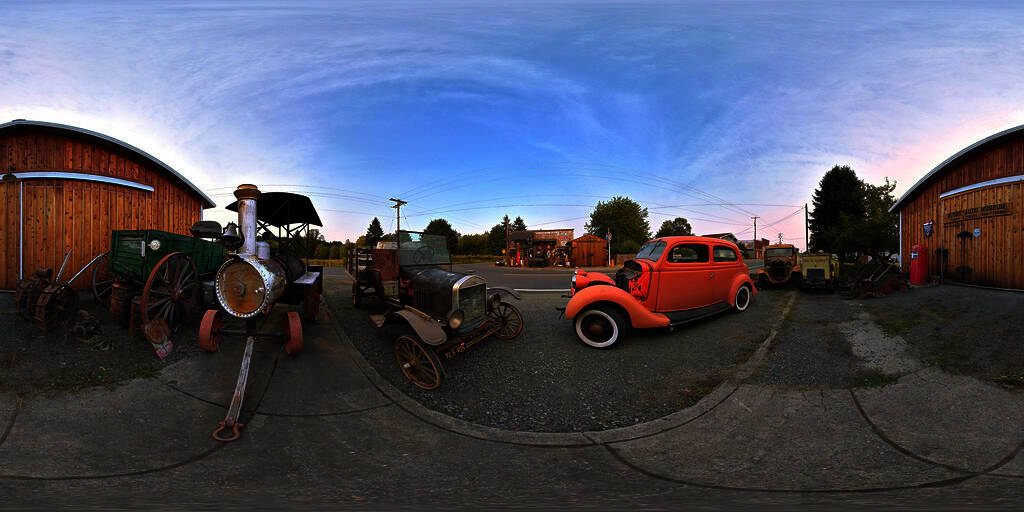
\includegraphics[width=0.4\textwidth]{imagenes/chapter3/Pano360/stripped-46549510}}
    \subfloat{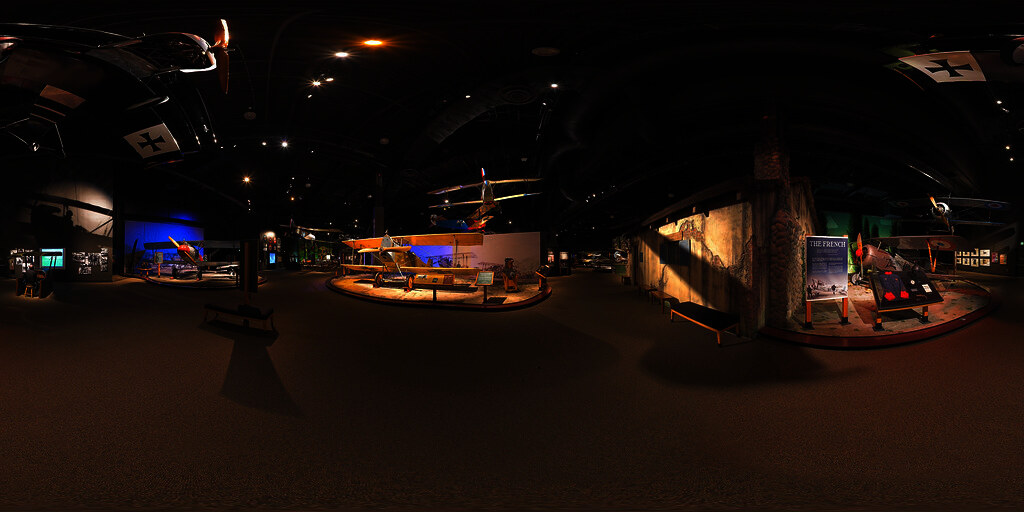
\includegraphics[width=0.4\textwidth]{imagenes/chapter3/Pano360/stripped-50535259}}
  \end{center}
  \caption{Ejemplos de escenas panorámicas de Pano360~\footcite{SPEC}}
\end{figure}
\end{frame}

\begin{frame}
  \frametitle{Generación de datos a partir de panorámicas}
\begin{figure}[!ht]
  \begin{center}
    \subfloat{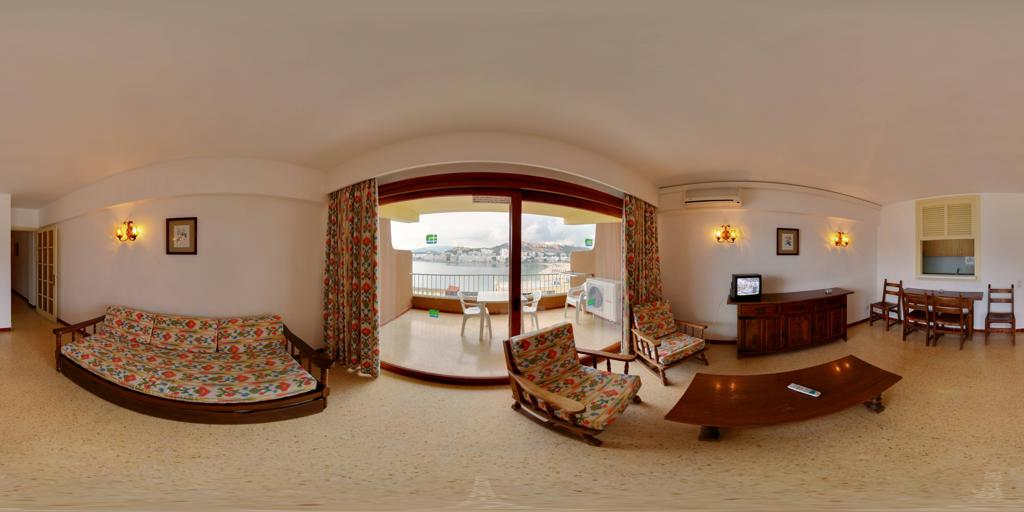
\includegraphics[width=0.4\textwidth]{imagenes/chapter3/Calib/pano_acizdacpcaveub.jpg}}\hfil
    \subfloat{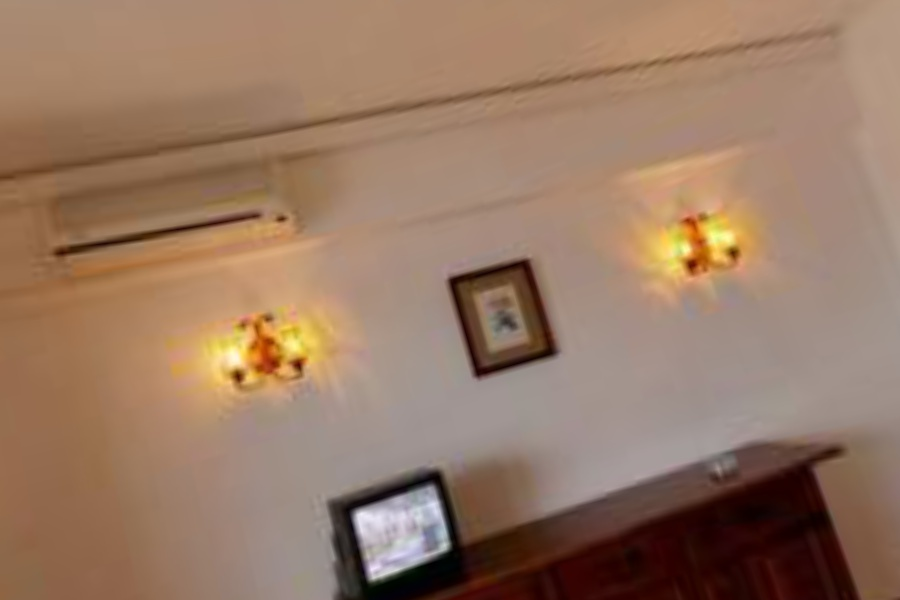
\includegraphics[width=0.25\textwidth]{imagenes/chapter3/Calib/pano_acizdacpcaveub.jpg-4.jpg}}
    \subfloat{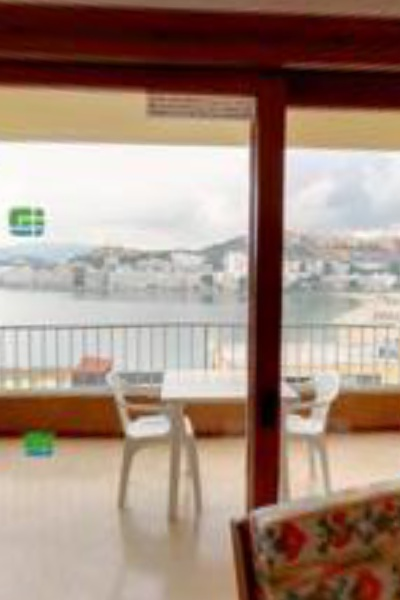
\includegraphics[width=0.15\textwidth]{imagenes/chapter3/Calib/pano_acizdacpcaveub.jpg-5.jpg}}
    \subfloat{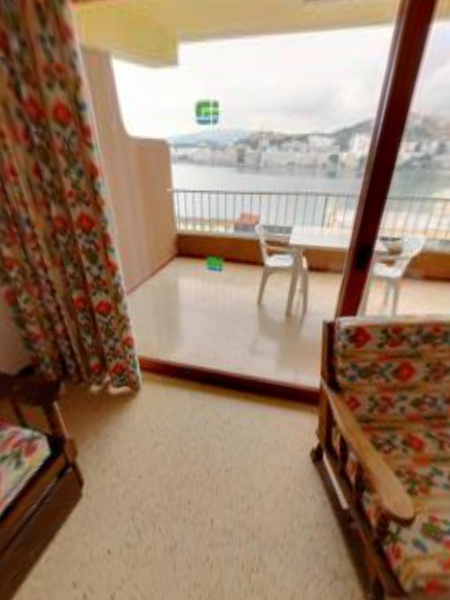
\includegraphics[width=0.15\textwidth]{imagenes/chapter3/Calib/pano_acizdacpcaveub.jpg-6.jpg}}
  \end{center}
  \caption[Ejemplo de imágenes obtenidas de una escena panorámica utilizando el algoritmo de~\footcite{CalibDataGeneration}.]{
  Ejemplo de imágenes obtenidas de una escena panorámica utilizando el algoritmo de~\footcite{CalibDataGeneration}.
  En este caso, dada una imagen panorámica de SUN360~\footcite{SUN360}, se extraen 3 recortes con parámetros de cámara diferentes.
}
\end{figure}
\end{frame}

\subsection{Datos de validación}
\begin{frame}
  \frametitle{Datos de validación: IdentAI}
\begin{figure}[!ht]
  \begin{itemize}
    \item Un total de 652 fotogramas válidos, con un total de 12 sujetos de diferentes estaturas en 4 escenas diferentes.
  \end{itemize}
\begin{center}
    \subfloat{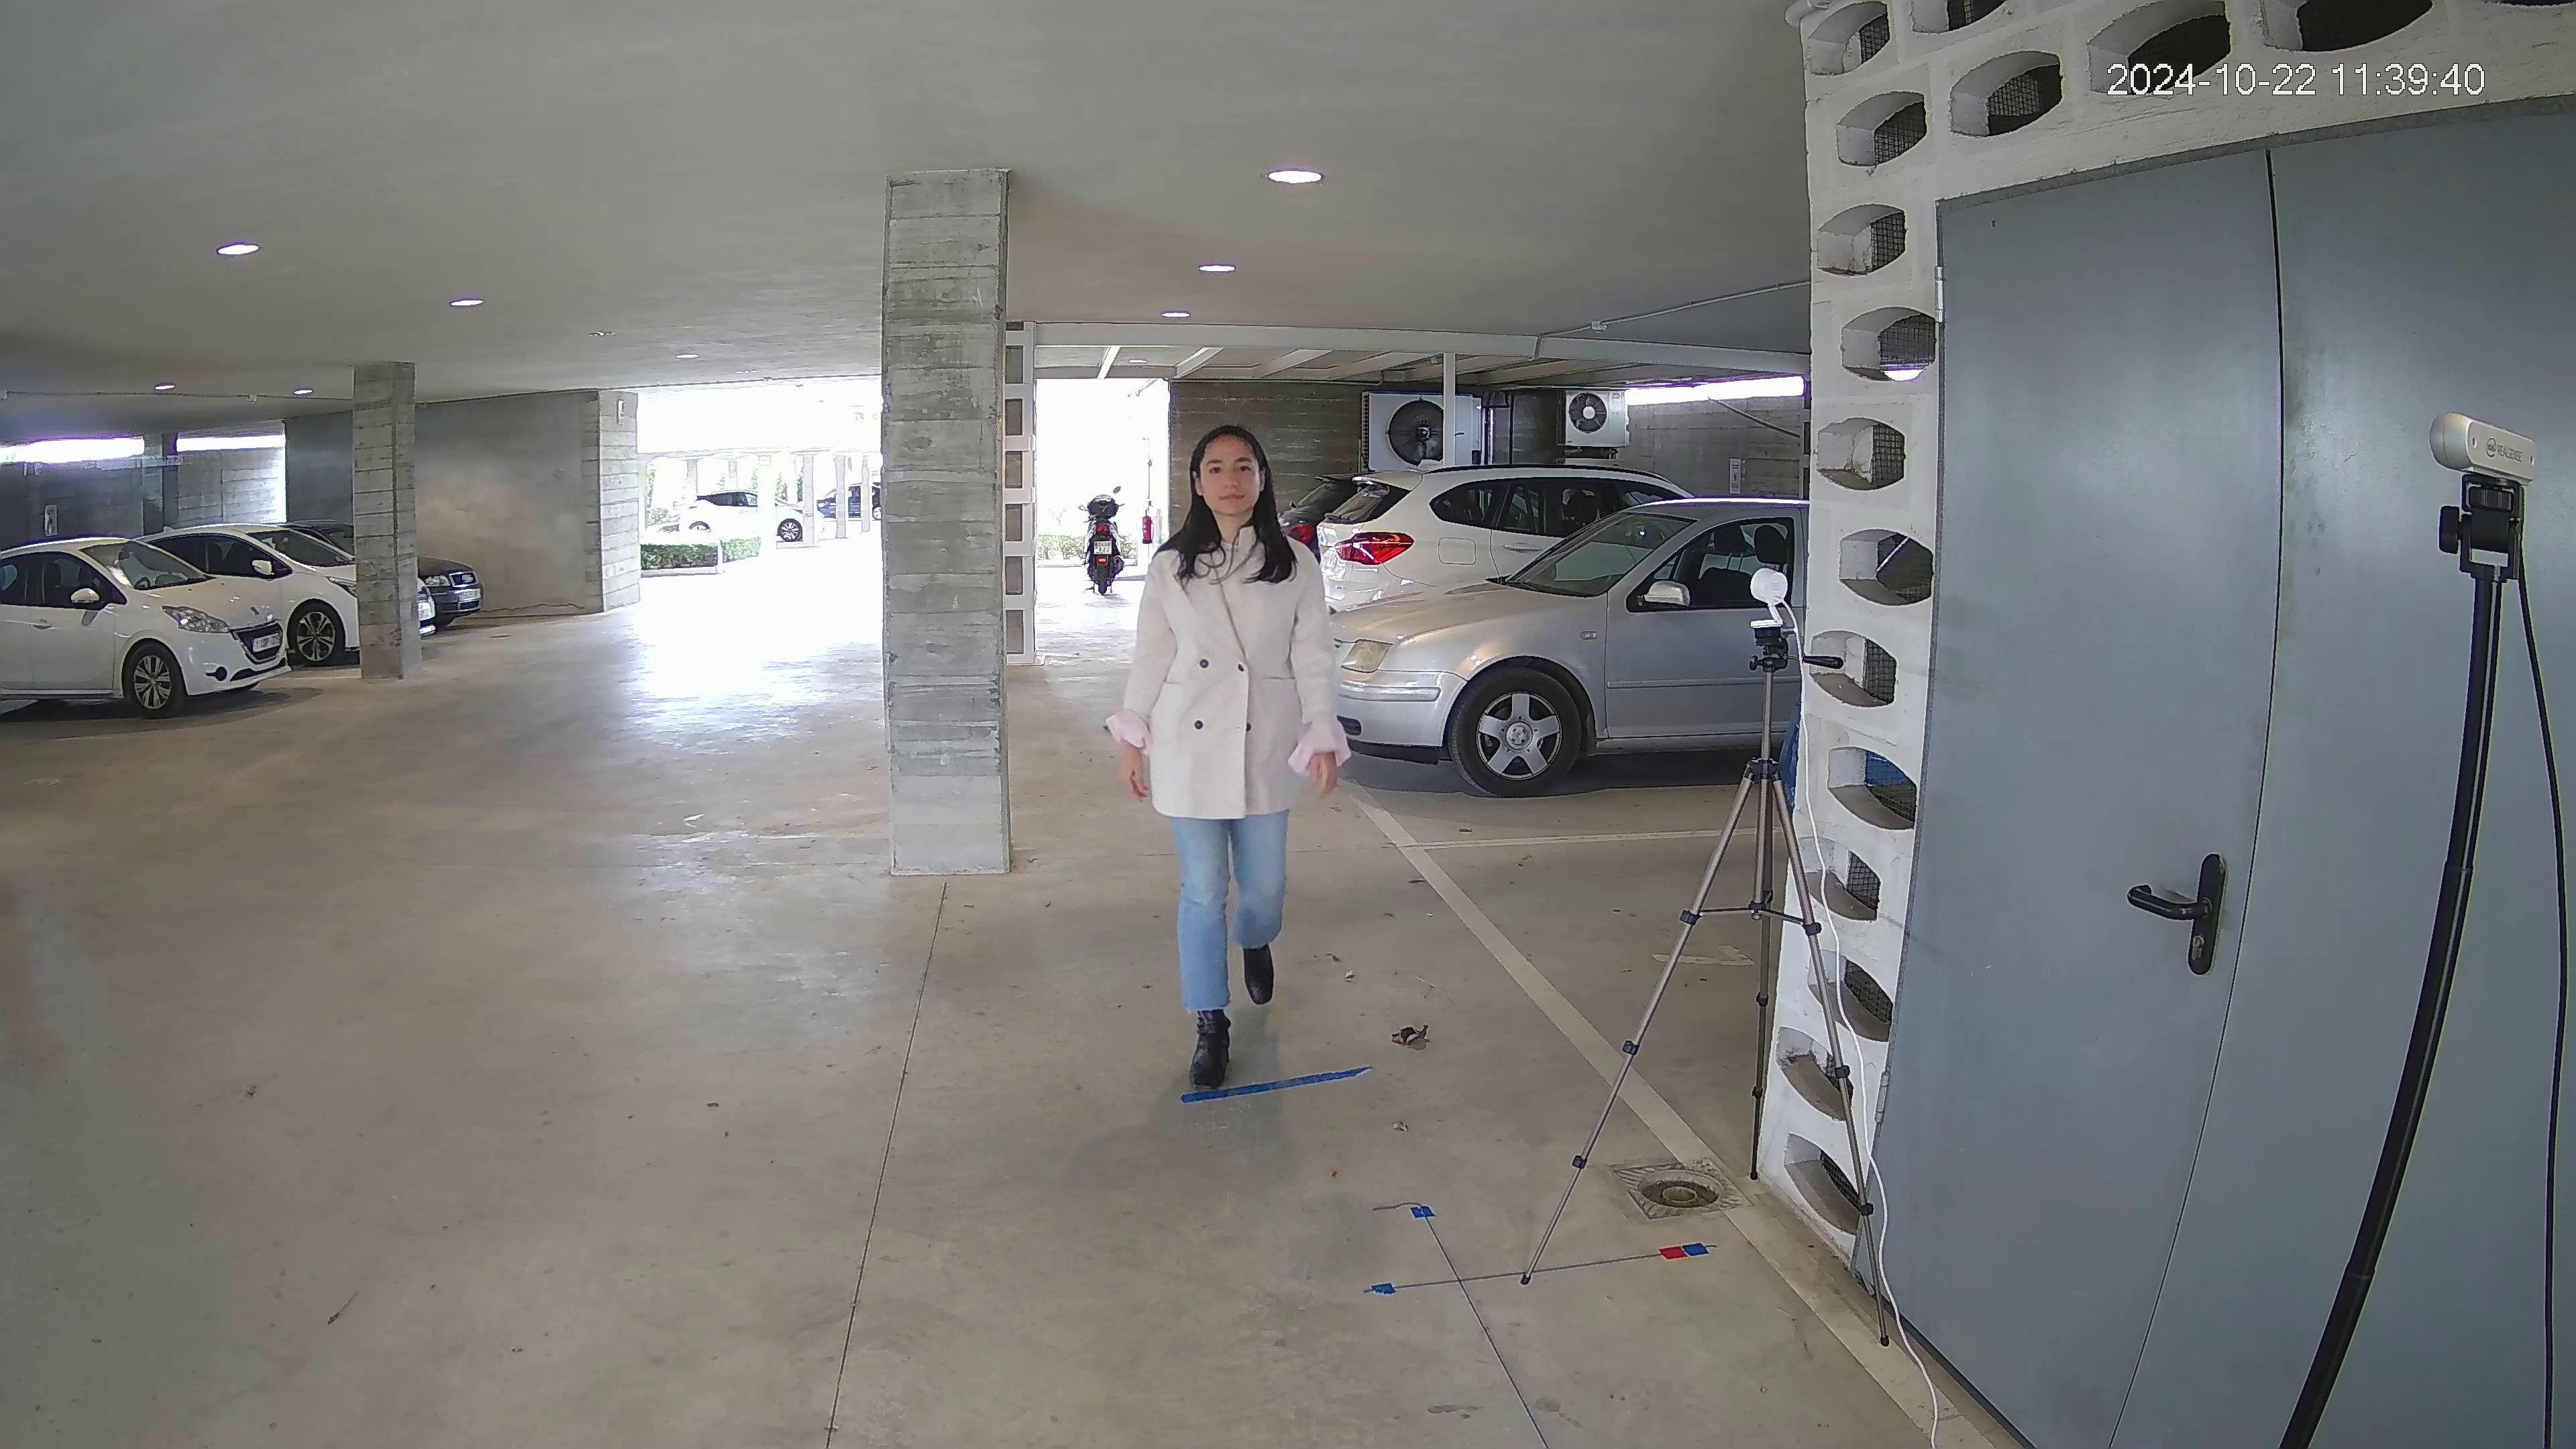
\includegraphics[width=0.35\textwidth]{imagenes/chapter3/ParkingLot.jpg}}
    \subfloat{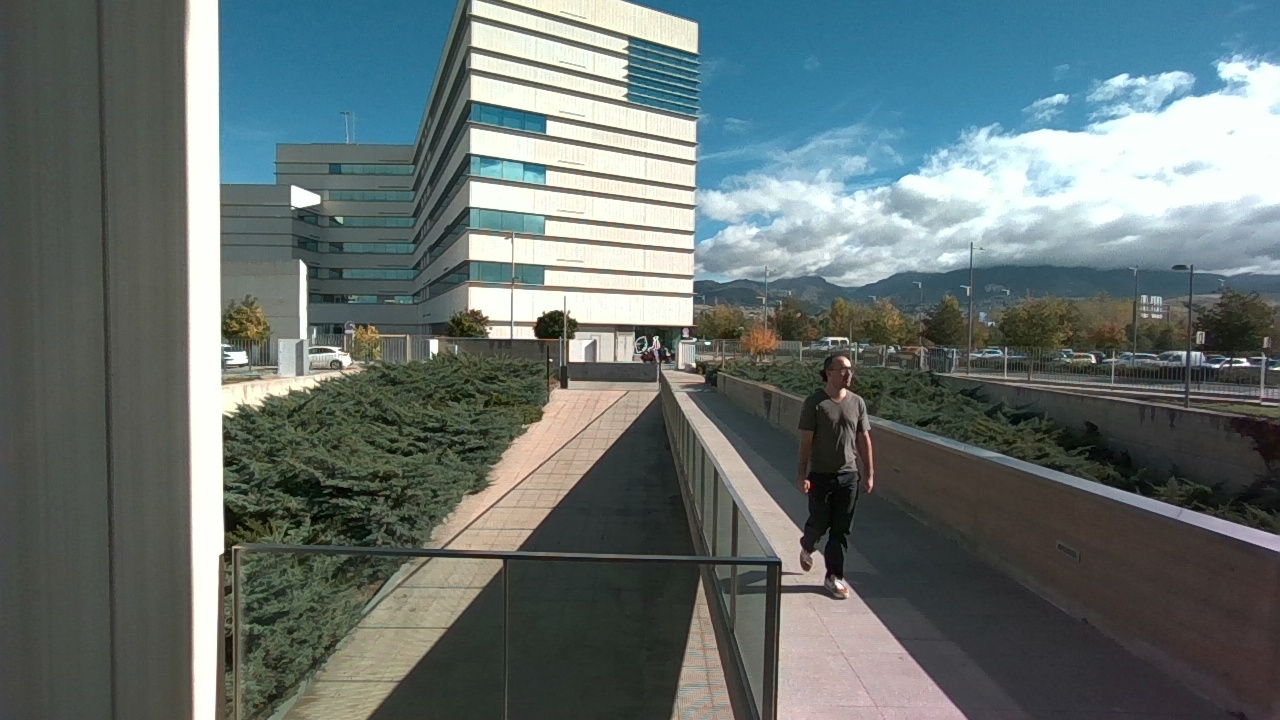
\includegraphics[width=0.35\textwidth]{imagenes/chapter3/EntranceRamp.jpg}}
    \subfloat{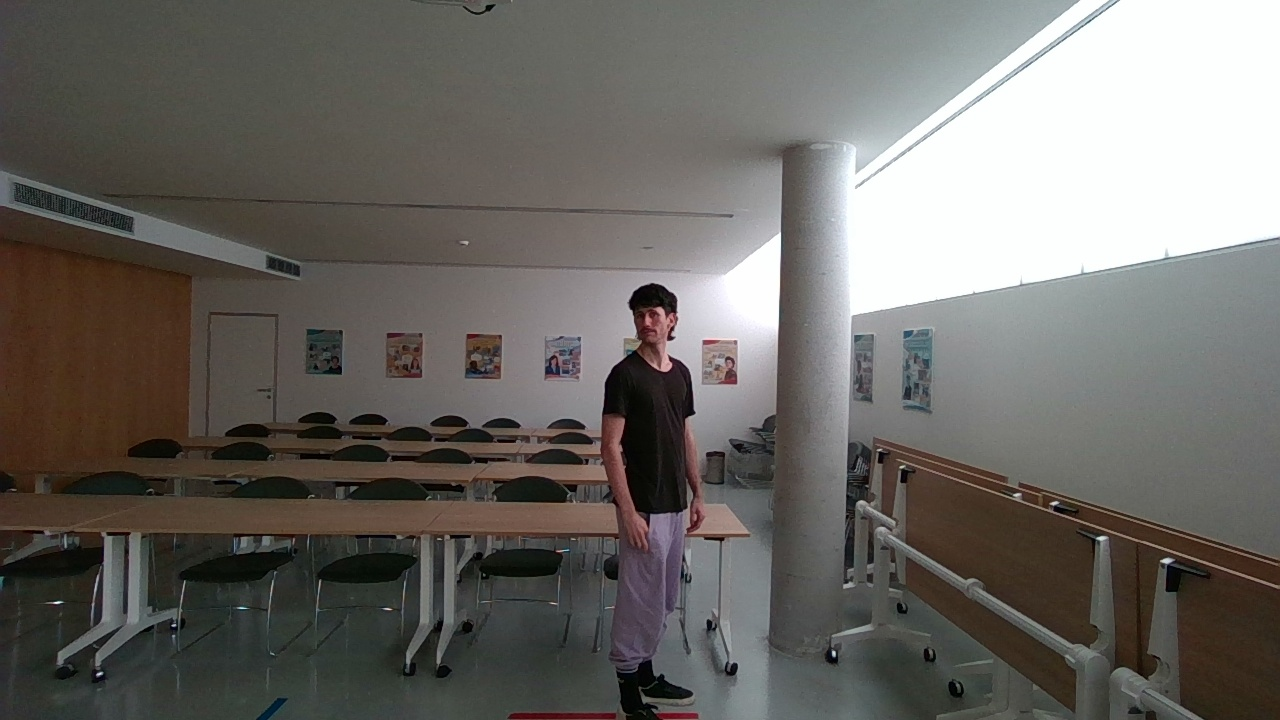
\includegraphics[width=0.35\textwidth]{imagenes/chapter3/SeminarRoom.jpg}}\\
\end{center}
\caption{Ejemplo de grabaciones del conjunto de datos IdentAI~\footcite{panacea2026}, realizadas en diferentes ubicaciones.}
\end{figure}
\end{frame}

\begin{frame}
\begin{itemize}
\item Se han seleccionado únicamente aquellas imágenes en las que la persona aparece completamente visible y en posición erguida.
\end{itemize}
\begin{table}[!htp]
  \scriptsize
  \centering
\begin{tabular}{|c|c|c|}
\hline
\rowcolor[HTML]{FFCB2F}
\textbf{Sujeto} & \textbf{Altura (cm)} & \textbf{Fotogramas} \\
\hline
idai001 & 162 & 56 \\
\hline
idai002 & 160 & 77 \\
\hline
idai003 & 184 & 4 \\
\hline
idai006 & 180 & 90 \\
\hline
idai007 & 169 & 65 \\
\hline
idai008 & 175 & 51 \\
\hline
idai009 & 178 & 4 \\
\hline
idai010 & 192 & 131 \\
\hline
idai011 & 174 & 6 \\
\hline
idai012 & 170 & 78 \\
\hline
idai014 & 174 & 49 \\
\hline
idai015 & 168 & 41 \\
\hline
\end{tabular}
\caption[Características descriptivas de los individuos del conjunto de datos IdentAI~\footcite{panacea2026}.]{
  Características descriptivas de los individuos del conjunto de datos IdentAI~\footcite{panacea2026}.
}
\end{table}
\end{frame}

\begin{frame}
  \frametitle{Datos de validación: KITTI}
  \begin{itemize}
    \item Se filtra el conjunto de imágenes por aquellas que contengan al menos una persona completamente visible.
  \end{itemize}
\begin{figure}[!ht]
  \begin{center}
    \subfloat{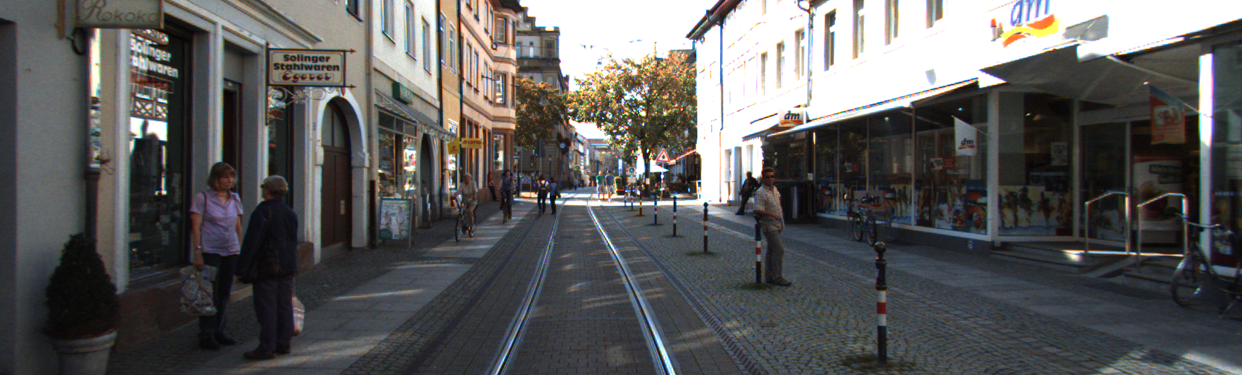
\includegraphics[width=0.7\textwidth]{imagenes/chapter3/Kitti/000073.png}}
    %\subfloat{
\includegraphics[width=0.6\textwidth]{imagenes/chapter4/Kitti/000074.png}}
  \end{center}
  \caption[Ejemplo de escena etiquetada de KITTI~\footcite{Kitti}.]{
    Ejemplo de escena etiquetada de KITTI~\footcite{Kitti}.
}
\end{figure}
\end{frame}

\begin{frame}
  \frametitle{Método clásico: retroproyección 2D a 3D.}
  \begin{itemize}
    \item Se utiliza la matriz de proyección de la cámara y una referencia conocida
      para estimar la posición 3D de los puntos de la imagen.
    \item Tras posicionar en la escena los pies y la cabeza, se estima la altura del objeto.
  \end{itemize}
\begin{figure}[!ht]
  \begin{center}
    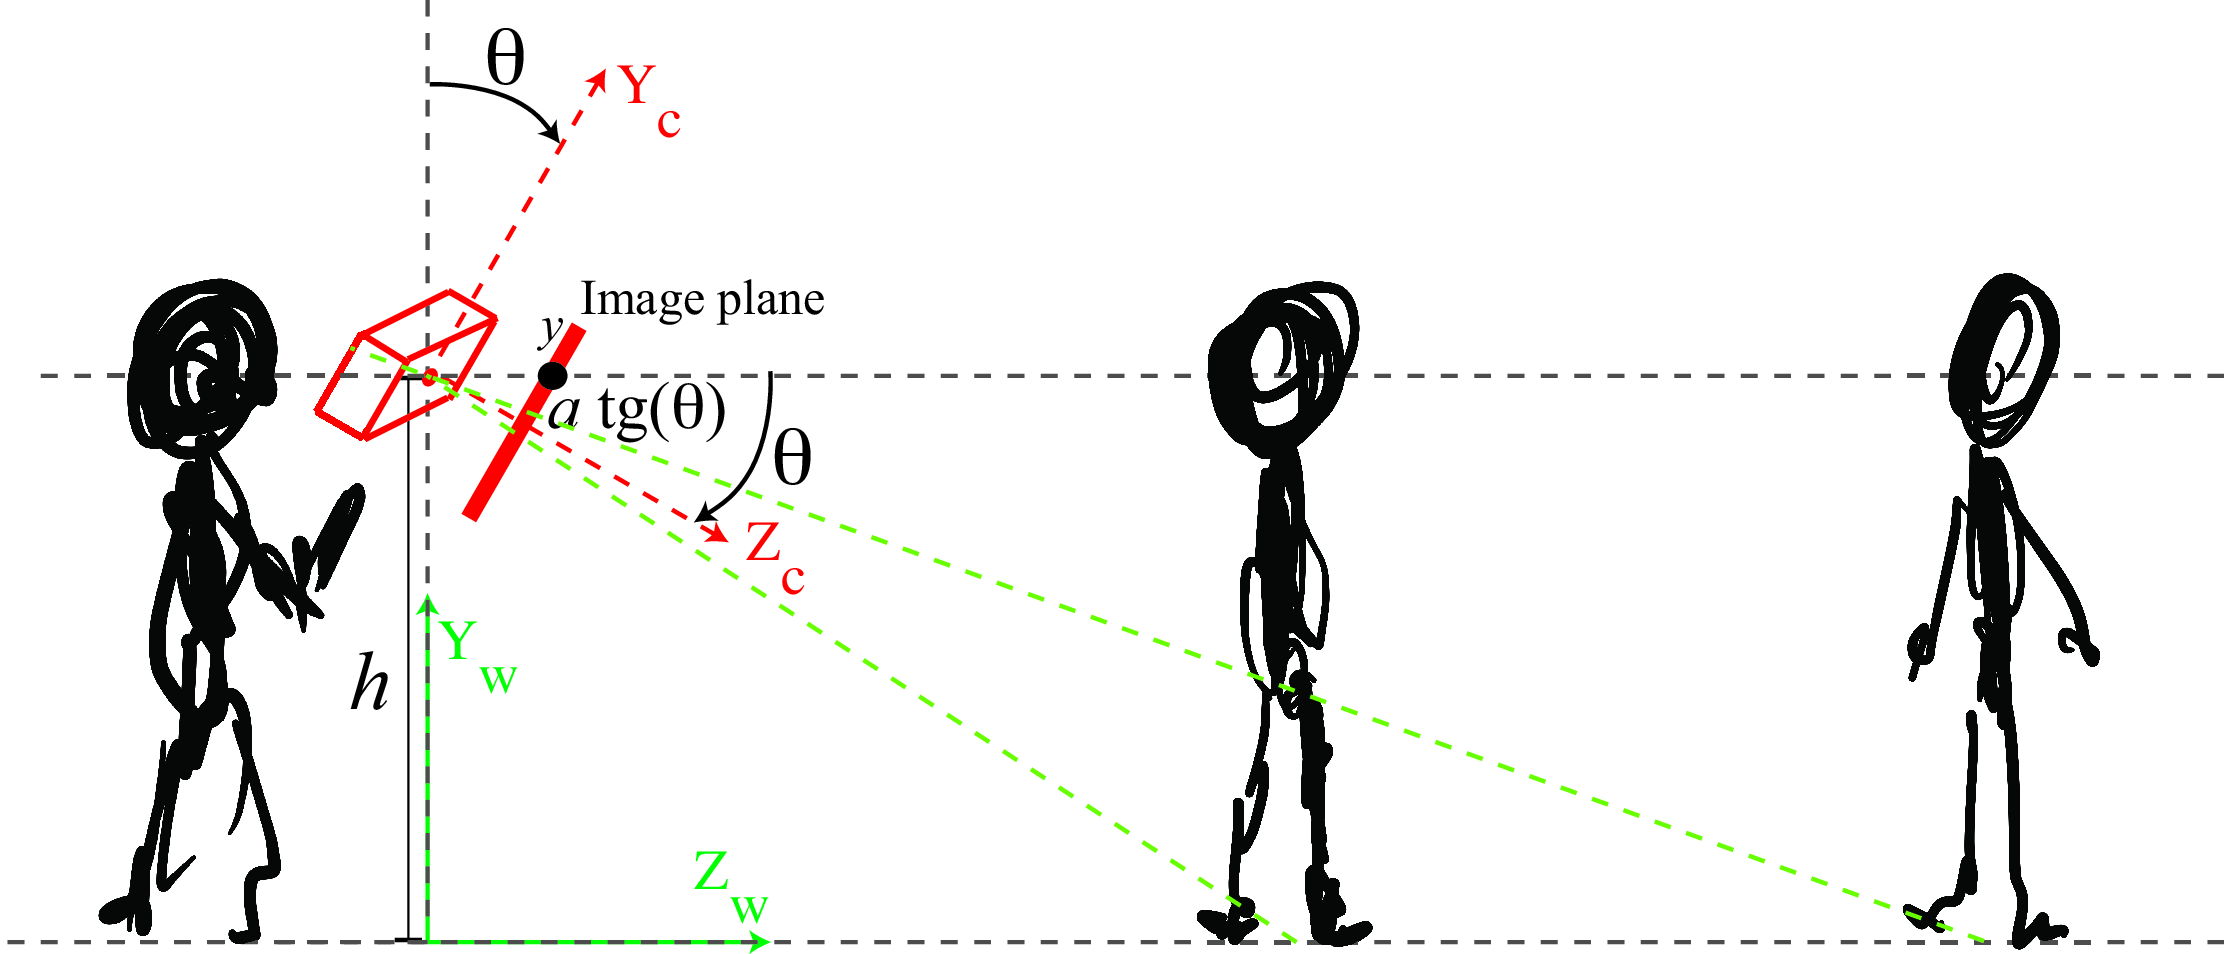
\includegraphics[width=0.6\textwidth]{imagenes/chapter3/camera-backprojection.png}
  \end{center}
  \caption[Procedimiento de retroproyección 3D para estimación de altura~\footcite{VisionBookMIT}.]{
    Procedimiento de retroproyección 3D para estimación de altura~\footcite{VisionBookMIT}.
}
\end{figure}
\end{frame}

\note{
  A partir de una referencia conocida, como la altura de la cámara respecto al plano del suelo ($Y_w$) o la
  distancia al sujeto en el eje de profundidad ($Z_w$), junto con la orientación de la cámara descrita por sus ángulos
  de rotación (por ejemplo el de inclinación, $\theta$), es posible calcular el rayo de visión asociado a
  un punto de la imagen, por ejemplo el de los pies, desde el sistema de coordenadas de la cámara al sistema de coordenadas del mundo.
  Posteriormente, se utiliza la referencia conocida para calcular el factor de escala que permite situar
  el punto de intersección del rayo que parte del centro óptico de la cámara ($Z_c$) sobre el plano del suelo
  en los pies del individuo. Una vez localizado este punto de referencia, la retroproyección del punto asociado
  a la cabeza permite estimar la altura del sujeto.
}

\subsection{Entorno}
\begin{frame}
  \frametitle{Tecnologías utilizadas}
  \begin{table}[htp]
      \begin{tabular}{cccc}
        \begin{minipage}{.2\textwidth}
          
\includegraphics[width=\textwidth]{imagenes/chapter3/tech/Python}
        \end{minipage}
                                  &
        \begin{minipage}{.2\textwidth}
          
\includegraphics[width=.65\textwidth]{imagenes/chapter3/tech/d2}
        \end{minipage}
                                  &
        \begin{minipage}{.2\textwidth}
          
\includegraphics[width=\textwidth]{imagenes/chapter3/tech/Pytorch}
        \end{minipage}
                                  &
        \begin{minipage}{.2\textwidth}
          
\includegraphics[width=.6\textwidth]{imagenes/chapter3/tech/OpenCV}
        \end{minipage}
                                  \\
        \begin{minipage}{.2\textwidth}
          
\includegraphics[width=\textwidth]{imagenes/chapter3/tech/Numpy}
        \end{minipage}
                                                        &
        \begin{minipage}{.2\textwidth}
          
\includegraphics[width=.9\textwidth]{imagenes/chapter3/tech/Scikit}
        \end{minipage}
                                                        &
        \begin{minipage}{.2\textwidth}
          
\includegraphics[width=.9\textwidth]{imagenes/chapter3/tech/Polars}
        \end{minipage}
        &
        \begin{minipage}{.2\textwidth}
          
\includegraphics[width=.55\textwidth]{imagenes/chapter3/tech/pandas}
        \end{minipage} \\
                                                        &
        \begin{minipage}{.2\textwidth}
          
\includegraphics[width=.9\textwidth]{imagenes/chapter3/tech/Nvidia}
        \end{minipage}
                                                        &
        \begin{minipage}{.2\textwidth}
          
\includegraphics[width=.9\textwidth]{imagenes/chapter3/tech/Colab}
        \end{minipage}
                                                        &
                                                        \\
      \end{tabular}
  \end{table}
\end{frame}

\note{
Para el desarrollo y ejecución de los modelos fue necesario el uso de
la librería de DL Pytorch junto con las librerías CUDA para poder ejecutar
los modelos en las tarjetas gráficas de NVIDIA. Para los cálculos numéricos y
el manejo de datos se utilizaron Numpy y Polars. Teniendo en cuenta que para el
cálculo de las métricas hemos utilizado la librería de scikit-learn.
Para la visualización y fácil manipulación de las nubes de puntos se hizo uso
de la librería de Open3D y Pyntcloud.
}



\note{}
